\documentclass[12pt,letterpaper,titlepage]{book}

\usepackage{amsmath}
\usepackage{amsfonts}
\usepackage{pgfplots}
\usepackage{siunitx}

\DeclareMathOperator{\arccot}{arccot}
\DeclareMathOperator{\arcsec}{arcsec}

\title{AP Calculus BC Midterm\\Study Guide}
\author{Taylor Blau}
\date{January, 2016}

\begin{document}

\maketitle
\tableofcontents

\chapter{Basic Identities}
\section{Basic Derivatives}
\begin{align*}
  \frac{d}{dx}[cu]=cu' &&
  \frac{d}{dx}[u\pm v]=u' \pm v' &&
  \frac{d}{dx}[uv]=uv'+vu' \\
  \frac{d}{dx}\left[\frac{u}{v}\right]=\frac{vu'-uv'}{u^2} &&
  \frac{d}{dx}[c]=0 &&
  \frac{d}{dx}[u^n]=nu^{n-1}u' \\
  \frac{d}{dx}[x]=1 &&
  \frac{d}{dx}[|u|]=\frac{u}{|u|}u' &&
  \frac{d}{dx}[\ln{u}]=\frac{u'}{u} \\
  \frac{d}{dx}[e^u]=e^uu' &&
  \frac{d}{dx}[\log_{a}u]=\frac{u'}{\ln{a}u} &&
  \frac{d}{dx}[a^u]=(\ln{a})a^uu' \\
  \frac{d}{dx}[\sin{u}]=\cos{u}u' &&
  \frac{d}{dx}[\cos{u}]=-\sin{u}u' &&
  \frac{d}{dx}[\tan{u}]=\sec^2{u}u' \\
  \frac{d}{dx}[\cot{u}]l=-\csc^2{u}u' &&
  \frac{d}{dx}[\sec{u}]=-(\sec{u}\tan{u})u' &&
  \frac{d}{dx}[\csc{u}]=-(\csc{u}\cot{u})u' \\
\end{align*}

\section{Basic Integrals}
\begin{align*}
  \int kf(u) du = k\int f(u) du &&
  \int [f(u) \pm g(u)] du = \int f(u) du \pm \int g(u) du \\
  \int du = u + C &&
  \int u^n du = \frac{u^{n+1}}{n+1} + C \\
  \int \frac{1}{u} du = \ln{|u|} + C &&
  \int e^u du = e^u + C \\
  \int a^u du = \frac{a^u}{\ln{a}} + C &&
  \int \sin{u} du = -\cos{u} + C \\
  \int \cos{u} du = \sin{u} + C &&
  \int \tan{u} du = -\ln{\cos{u}} + C \\
  \int \cot{u} du = \ln{\sin{u}} + C &&
  \int \sec{u} du = \ln{\sec{u}+\tan{u}} + C \\
  \int \csc{u} du = -\ln{\csc{u}+\cot{u}} + C &&
  \int \sec^2{u} du = \tan{u} + C \\
  \int \csc^2{u} du = -\cot{u} + C &&
  \int \sec{u}\tan{u} du = \sec{u} + C \\
  \int \csc{u}\cot{u} du = -\csc{u} + C &&
  \int \frac{1}{a^2+u^2} du = \frac{1}{a}\arctan{\frac{u}{a}} + C \\
  \int \frac{1}{\sqrt{a^2-u^2}} du = \arcsin{\frac{u}{a}} + C &&
  \int \frac{1}{u\sqrt{u^2-a^2}} du = \frac{1}{a}\arcsec{\frac{|u|}{a}} + C
\end{align*}

\section{Basic Trigonometry}
\subsection{Definitions}
\begin{align*}
  \sin\theta=\frac{\text{opp}}{\text{hyp}} &&
  \cos\theta=\frac{\text{adj}}{\text{hyp}} &&
  \tan\theta=\frac{\text{opp}}{\text{adj}} \\
  \csc\theta=\frac{\text{hyp}}{\text{opp}} &&
  \sec\theta=\frac{\text{hyp}}{\text{adj}} &&
  \cot\theta=\frac{\text{adj}}{\text{hyp}} \\
\end{align*}

\subsection{Reciporocal Identities}
\begin{align*}
  \sin\theta=\frac{1}{\csc\theta} &&
  \cos\theta=\frac{1}{\sec\theta} &&
  \tan\theta=\frac{1}{\cot\theta} \\
  \csc\theta=\frac{1}{\sin\theta} &&
  \sec\theta=\frac{1}{\cos\theta} &&
  \cot\theta=\frac{1}{\tan\theta} \\
\end{align*}

\subsection{Double-Angle Formulas}
\begin{align*}
  \sin{2u} &= 2\sin{u}\cos{u} \\
  \cos{2u} &= \cos^2{u}-\sin^2{u} \\
           &= 2\cos^2{u}-1 \\
           &= 1-2\sin^2{u} \\
  \tan{2u} &= \frac{2\tan{u}}{1-\tan^2{u}}
\end{align*}

\subsection{Power-Reducing Formulas}
\begin{align*}
  \sin^2{u} &= \frac{1-\cos2u}{2} \\
  \cos^2{u} &= \frac{1+\cos2u}{2} \\
  \tan^2{u} &= \frac{1-\cos2u}{1+\cos2u}
\end{align*}

\subsection{Pythagorean Identities}
\begin{align*}
  \sin^2\theta+\cos^2\theta=1 \\
  1+\tan^2\theta=\sec^2\theta \\
  1+\cot^2\theta=\csc^2\theta
\end{align*}

\subsection{Sum and Difference Formulas}
\begin{align*}
  \sin{u \pm v} &= \sin{u}\cos{v} \pm \cos{u}\sin{v} \\
  \cos{u \pm v} &= \cos{u}\cos{v} \mp \sin{u}\sin{v} \\
  \tan{u \pm v} &= \frac{\tan{u}\pm\tan{v}}{1\mp\tan{u}\tan{v}}
\end{align*}


\chapter{Unit 1}
\section{Plane Curves \& Parametrics}
\subsection{Definition}
Typically, functions come in rectangular form, meaning $x$ is the independent
variable, and $y$ is dependent upon it. These functions look recognizable:
$y=\ln(x)$.

To track more things, or place a function into a seperate independent variable,
parametrics are used. When using parametrics, one function is given for every
graphed dimension. For example: $x=f(t)$, $y=f(t)$ or $x=f(\theta)$,
$y=f(\theta)$.

In the above example, $x(t)$ and $y(t)$ are the parametric equations and $t$ is
the parameter. The set of points $(x, y)$ obtained as $t$ varries over the
interval on which it is defined, is the graph of the parametric equation.

\subsection{De-parameterizing}
\begin{description}
  \item[Table] A table of values can be created where $t$ varries independently,
    and $(x(t), y(t))$ are the output values.
  \item[Algebraic Simplification] $x(t)$ can be simplified in terms of $y$ and
    substituted back into $y(t)$ to obtain a function.
  \item[Trigonometric Simplification] Trigonometric identities (such as
    $\sin^2\theta + \cos^2\theta = 1$, etc.) may be used to simplify the
    parameter functions.
\end{description}

\subsection{Parameterizing}
To obtain the parametric curve of the rectangular equation, the
following process is implemented:

\begin{enumerate}
  \item Let $x(t) = t$, and write $y(t)$ in terms of $x(t)$.
  \item Write both $x$ and $y$ in terms of $t$ and $m=\frac{dy}{dx}$.
\end{enumerate}

An example is shown below for the curve $y=1-x^2$:

\begin{align*}
  x(t) &= t\\
  y(t) &= 1-x^2\\
       &= 1-t^2\\\\
  m &= \frac{dy}{dx}=-2x\\\\
  x &= \frac{-m}{2}\\\\
  y &= 1-x^2\\
    &= 1-(\frac{-m}{2})^2\\
    &= 1-\frac{m^2}{4}
\end{align*}

\section{Parametric Equations and Calculus}
\subsection{The Derivative}
Suppose a parametric equation is given $x=f(t)$ and $y=g(t)$. The slope of that
equation is given to be:
\begin{equation}
  \frac{dy}{dx}=\frac{\frac{dy}{dt}}{\frac{dx}{dt}}
\end{equation}

The second derivative, therefore, of a parametric curve is given to be:
\begin{equation}\begin{aligned}
  \frac{d^2y}{dx^2} &=
  \frac{d}{dx}\left(\frac{\frac{dy}{dt}}{\frac{dx}{dt}}\right)\\
  &= \frac{d}{dx}\left(\frac{dy}{dx}\right)
\end{aligned}\end{equation}

\subsection{Arc Length}
Recall that the formula for arc length of a curve $h(x)$ over $[x_o, x_1]$ is:
\begin{equation}
  S = \int_{x_0}^{x_1} \sqrt{1+\left[h'(x)\right]^2} dx\\
\end{equation}

Therefore making the arc length of a parametric curve the following:
\begin{align*}
  S &= \int_{x_0}^{x_1} \sqrt{1+\left[\frac{dy}{dx}\right]^2} dx\\
    &= \int_{x_0}^{x_1} \sqrt{1+\left[\frac{dy/dt}{dx/dt}\right]^2} dx\\
    &= \int_{x_0}^{x_1} \sqrt{\frac{(dx/dt)^2+(dy/dt)^2}{(dx/dt)^2}} dx\\
    &= \int_{x_0}^{x_1}
  \sqrt{\left(\frac{dx}{dt}\right)^2+\left(\frac{dy}{dt}\right)^2} dx\\
    &= \int_{x_0}^{x_1} \sqrt{[f'(t)]^2+[g'(t)]^2} dx\\
\end{align*}

\subsection{Areas of Rotation}
The revolution about the $x$-axis is given:
\begin{equation}
  S=2\pi\int_a^b
  g(t)\sqrt{\left(\frac{dx}{dt}\right)^2+\left(\frac{dy}{dt}\right)^2} dt
\end{equation}

and the area about the $y$-axis is given:
\begin{equation}
  S=2\pi\int_a^b
  f(t)\sqrt{\left(\frac{dx}{dt}\right)^2+\left(\frac{dy}{dt}\right)^2} dt
\end{equation}

\section{Vectors in the Plane}
Vectors are directed line segments that have no origin. Vectors have both
magnitude, and direction, such that any vector is the same no matter where they
start. Vectors are denoted as follows:
$$\vec{v}=\vec{PQ}$$

\subsection{Magnitude}
The magnitude of a vector $\vec{v}$ with the components $\langle x,y\rangle$ may
be calculated as follows:
\begin{equation}
  ||\vec{v}||=\sqrt{x^2+y^2}
\end{equation}

\subsection{Operations}
Let $\vec{u}=\langle u_1,u_2\rangle$ and $\vec{v}=\langle v_1,v_2\rangle$.
\begin{enumerate}
  \item The vector sum of $\vec{u}$ and $\vec{v}$ is $\langle u_1+v_1, u_2+v_2
    \rangle$.
  \item The scalar multiple of $c$ and $\vec{v}$ is $\langle cv_1, cv_2
    \rangle$.
  \item The negative of $\vec{v}$ is $\langle -v_1, -v_2 \rangle$.
  \item The difference of $\vec{u}$ and $\vec{v}$ is $\langle u_1-v_1, u_2-v_2
    \rangle$.
\end{enumerate}

To take the unit vector of a vector $\vec{v}$ in its direction, then the
following is calculated:
\begin{equation}
  \vec{u}=\frac{\vec{v}}{||\vec{v}||}=\frac{1}{||\vec{v}||}\vec{v}
\end{equation}

There are three standard unit vectors in $\mathbb{R}^3$ space:
\begin{description}
  \item[$\hat{i}$] = $\langle 1,0,0 \rangle$
  \item[$\hat{j}$] = $\langle 0,1,0 \rangle$
  \item[$\hat{k}$] = $\langle 0,0,1 \rangle$
\end{description}

\subsection{Space Coordinates and Vectors in Space}
Points in the $\mathbb{R}^2$ plane have coordinates of the form $(x,y)$. Points
in the $\mathbb{R}^3$ space have coordinates of the form $(x,y,z)$.

The distance between two such points takes the following form:
\begin{equation}
  d=\sqrt{(x_2-x_1)^2+(y_2-y_1)^2+(z_2-z_1)^2}
\end{equation}

Vectors in $\mathbb{R}^2$ take the form $\langle x,y,z \rangle$. All of the same
properties of vectors defined in $\mathbb{R}^2$ space apply here as well.

\section{The Dot Product}
The dot product determines information about the angle between two vectors. The
dot producted is calculated between two vectors $\vec{u}=\langle u_1,u_2
\rangle$ and $\vec{v}=\langle v_1,v_2 \rangle$ as follows:

\begin{equation}
  \vec{u} \cdot \vec{v} = u_1v_1 + u_2v_2
\end{equation}

\subsection{The Angle Between Two Vectors}
The dot product gives information about the angle between two non-zero vectors.
The following theorem is presented:
\begin{equation}
  \cos\theta = \frac{\vec{u}\cdot\vec{v}}{||\vec{u}||||\vec{v}||}
\end{equation}

\subsection{Direction Cosines}
The dot product can also be used to determine the angle between a vectors
components in $\mathbb{R}^3$ space and their respective planes of interest. For
example, for the vector $\vec{v} = \langle v_1,v_2,v_3 \rangle$, we can
determine the angle between each planar axis and the components of the vector.

The process is outlined below:
\begin{enumerate}
  \item Take the dot-product of a vector and a unit vector of magnitude $1$ in
    that plane (i.e., $\hat{i}$, $\hat{j}$, or $\hat{k}$).
  \item Apply the definition of the dot-product to determine the direction
    cosine.
\end{enumerate}

\begin{align}
  \cos\alpha &= \frac{v_1}{||\vec{v}||}\\
  \cos\beta  &= \frac{v_2}{||\vec{v}||}\\
  \cos\gamma &= \frac{v_3}{||\vec{v}||}
\end{align}

\subsection{Projections}
To project $\vec{u}$ onto $\vec{v}$ is to take the length of $\vec{u}$ in the
direction of $\vec{v}$. The notation is as follows below:

\begin{equation}
  \text{proj}_{\vec{v}}\vec{u}=
  \left(\frac{\vec{u}\cdot\vec{v}}{||\vec{v}||^2}\right)\vec{v}
\end{equation}

\subsubsection{Work}
\begin{align}
  W &= ||\text{proj}_{\vec{PQ}}\vec{F}||||\vec{PQ}|| \\
    &= \vec{F} \cdot \vec{PQ}
\end{align}

\section{The Cross Product}
Let $\vec{u}=\langle u_1,u_2,u_3 \rangle$ and $\vec{v}=\langle v_1,v_2,v_3
\rangle$. The cross product of $\vec{u}$ and $\vec{v}$ is said to be:
\begin{equation}
  \vec{u}\times\vec{v} = (u_2v_3-u_3v_2)\hat{i} - (u_1v_3-u_3v_1)\hat{j} +
  (u_1v_2-u_2v_1)\hat{k}
\end{equation}

Another way to calculate the cross product is with matricies:

\begin{equation}
  \begin{aligned}
    \vec{u}\times\vec{v} &= \begin{vmatrix}
      \hat{i} & \hat{j} & \hat{k} \\
      u_1     & u_2     & u_3 \\
      v_1     & v_2     & v_3
    \end{vmatrix} \\
  &= \begin{vmatrix}
    u_2 & u_3 \\
    v_2 & v_3 \\
  \end{vmatrix}\hat{i} -
  \begin{vmatrix}
    u_1 & u_3 \\
    v_1 & v_3 \\
  \end{vmatrix}\hat{j} +
  \begin{vmatrix}
    u_1 & u_2 \\
    v_1 & v_2 \\
  \end{vmatrix}\hat{k}\\
  &= (u_2v_3-u_3v_2)\hat{i} - (u_1v_3-u_3v_1)\hat{j} + (u_1v_2-u_2v_1)\hat{k}
  \end{aligned}
\end{equation}

\subsection{Algebraic Properties}
\begin{enumerate}
  \item $\vec{u}\times\vec{v}=-(\vec{v}\times\vec{u})$
  \item
    $\vec{u}\times(\vec{v}+\vec{w})=(\vec{u}\times\vec{v})+
    (\vec{u}\times\vec{w})$
  \item
    $c(\vec{u}\times\vec{v})=(c\vec{u})\times\vec{v}=\vec{u}\times(c\vec{v})$
  \item $\vec{u}\times0=0\times\vec{u}=0$
  \item $\vec{u}\times\vec{u}=0$
  \item $\vec{u}\dot(\vec{v}\times\vec{w}=(\vec{u}\times\vec{v})\cdot\vec{w}$
\end{enumerate}

\subsection{Geometric Properties}
\begin{enumerate}
  \item $\vec{u}\times\vec{v}$ is orthagonal to both $\vec{u}$ and $\vec{v}$
  \item $||\vec{u}\times\vec{v}||=||\vec{u}||||\vec{v}||\sin\theta$
  \item $\vec{u}\times\vec{v}=0$ only if $\vec{u}=c\vec{v}$
  \item $||\vec{u}\times\vec{v}||$ is the area of a parallelogram having
    $\vec{u}$ and $\vec{v}$ as adjacent sides.
\end{enumerate}

\subsection{The Triple Scalar Product}
\begin{equation}
  \vec{u}\cdot(\vec{v}\times\vec{w})=\begin{vmatrix}
    u_1 & u_2 & u_3 \\
    v_1 & v_2 & v_3 \\
    w_1 & w_2 & w_3
  \end{vmatrix}
\end{equation}

\subsubsection{Geometric Properties}
The volume of a parallelpiped with significant edges $\vec{u}$, $\vec{v}$, and
$\vec{w}$ is defined as:
\begin{equation}
  \begin{aligned}
    V &= |\vec{u}\cdot(\vec{v}\times\vec{w})| \\
      &= ||\text{proj}_{\vec{v}\times\vec{w}}||||\vec{v}\times\vec{w}|| \\
      &= \left|\frac
        {\vec{u}\cdot(\vec{v}\times\vec{w})}
        {||\vec{v}\times\vec{w}||}\right|
        ||\vec{v}\times\vec{w}|| \\
      &= |\vec{u}\cdot(\vec{v}\times\vec{w})|
  \end{aligned}
\end{equation}

\section{Lines and Planes in Space}
\subsection{Lines}
Given a line containing the point $P(x_1,y_1,z_1)$ in space parallel to the
vector $\vec{v}=\langle a,b,c \rangle$, the vector $\vec{v}$ is the direction
vector and the numbers $a$, $b$, and $c$ are direction numbers. One can surmise
that a line in space $L$ contains all points $Q(x,y,z)$ for which
$\vec{PQ}=c\vec{v}$.

\begin{equation}
  \begin{aligned}
    \vec{PQ} &= \langle x-x_1, y-y_1, z-z_1 \rangle \\
             &= \langle at, bt, ct \rangle \\
             &= t\vec{v}
  \end{aligned}
\end{equation}

The following parametric equations are generated:
\begin{align}
  x=x_1+at \\
  y=y_1+at \\
  z=z_1+at
\end{align}

and the symmetric equation of the line can be generated by eliminating the
parameter:

\begin{equation}
  \frac{x-x_1}{a} = \frac{y-y_1}{b} = \frac{z-z_1}{c}
\end{equation}

\subsection{Planes}
Consider a plane in space containing the point $P(x_1,y_1,z_1)$ and
$Q(x_2,y_2,z_2)$. There is some vector in the plane, therefore, $\vec{v}=\langle
(x_2-x_1,y_2-y_1,x_2-z-1 \rangle$, and some other vector $\vec{n}$ such that
$\vec{v}\cdot\vec{n}=0$. Let $\vec{n}=\langle a,b,c \rangle$.

It can be said that:
\begin{equation}
  \begin{aligned}
    \vec{n}\cdot\vec{PQ} &= 0\\
    \langle a,b,c \rangle \cdot \langle x-x_1, y-y_1, z-z_1 \rangle &= 0\\
    a(x-x_1)+b(y-y_1)+c(z-z_1) &= 0\\
    ax+by+cz+d &= 0
  \end{aligned}
\end{equation}

To generate the vector $\vec{n}$, it is useful to generate two vectors in the
plane $\vec{u}$ and $\vec{v}$ and then take their cross product to obtain
$\vec{n}$ such that $\vec{u}\times\vec{v}=\vec{n}$.

The dot-product can be used to determine the angle between two planes by using
their normal vectors $\vec{n_1}$ and $\vec{n_2}$.
\begin{equation}
  \cos\theta=\frac{|\vec{n_1}\cdot\vec{n_2}|}{||\vec{n_1}||||\vec{n_2}||}
\end{equation}

\subsubsection{Distance between a Point and a Plane}
The distance $D$ between a point $Q(x_0,y_0,z_0)$ (not in the plane) and $P$ (in
the plane with the direction numbers $A$, $B$, $C$, and $D$) is:
\begin{equation}
  \begin{aligned}
    D &= ||\text{proj}_{\vec{n}}\vec{PQ}|| \\
      &= \frac{\vec{PQ}\cdot\vec{n}}{||\vec{n}||} \\
      &= \frac{|ax_0+by_0+cz_0+d|}{\sqrt{a^2+b^2+c^2}}
  \end{aligned}
\end{equation}

\subsubsection{Distance between a Point and a Line}
The distance $D$ between a point $Q$ and a line in space containing the point
$P$ is:
\begin{equation}
  D = \frac{||\vec{PQ}\times\vec{u}||}{||\vec{u}||}
\end{equation}

\section{Vectored-Valued Functions}
Vectored valued functions are functions that produced vectors ($\langle x,y,z
\rangle$ in $\mathbb{R}^3$ space, $\langle x,y \rangle$ in $\mathbb{R}^2$ space).

Vectored valued functions are denoted as follows:

\begin{equation}
  \vec{r}(t) = \langle \vec{f}(t), \vec{g}(t), \vec{h}(t) \rangle
\end{equation}

These functions are drawn as normal curves, such that each point on the curve
$P(x,y)$ represents a vector $\vec{v} = \langle x,y \rangle$. Just like normal
parametric curves, they have direction or orientation.

The limits of these functions may be taken as follows:
\begin{equation}
  \lim_{x\to{a}} \vec{r}(t) =
    \left[\lim_{x\to{a}}\vec{f}(t)\right]\hat{i} +
    \left[\lim_{x\to{a}}\vec{g}(t)\right]\hat{j} +
    \left[\lim_{x\to{a}}\vec{h}(t)\right]\hat{k}
\end{equation}

\section{Calculus of Vectored-Valued Functions}
\subsection{Differentiation}
The derivative of a vectored-valued function $\vec{r}(t)$ is given as:
\begin{equation}
  \vec{r}'(t)=\lim_{\Delta{t}\to{0}}
    \frac{\vec{r}(t+\Delta{t})-\vec{r}(t)}{\Delta{t}}
\end{equation}

Such that:
\begin{equation}
  \vec{r}'(t) = \frac{d}{dt}\vec{f}(t) +
                \frac{d}{dt}\vec{g}(t) +
                \frac{d}{dt}\vec{h}(t)
\end{equation}

\subsection{Properties}
\begin{enumerate}
  \item $$\frac{d}{dt}[\vec{r}(t)\cdot\vec{u}(t)] = \vec{r}(t)\cdot\vec{u}'(t) +
                                                    \vec{u}(t)\cdot\vec{r}'(t)$$
  \item $$\frac{d}{dt}[\vec{r}(t)\times\vec{u}(t)]=\vec{r}(t)\times\vec{u}'(t) +
                                                   \vec{u}(t)\times\vec{r}'(t)$$
\end{enumerate}

\subsection{Integration}
The integral of a vectored-valued function $\vec{r}(t)$ is given as: (note, this
applies to vector-valued functions in $\mathbb{R}^2$ and $\mathbb{R}^3$ for both
definite and indefinite integrals)
\begin{equation}
  \int \vec{r}(t) dt = \left(\int \vec{f}(t) dt\right)\hat{i} +
                       \left(\int \vec{g}(t) dt\right)\hat{j} +
                       \left(\int \vec{h}(t) dt\right)\hat{k}
\end{equation}

\section{Velocity \& Acceleration}
Let $\vec{a}(t)$, $\vec{v}(t)$ and $\vec{r}(t)$ represent the acceleration,
velocity, and position of an object in $\mathbb{R}^2$ or $\mathbb{R}^3$
respectively.
\begin{equation}
  \vec{a}(t) = \frac{d}{dt}\left[\vec{v}(t)\right]
             = \frac{d^2}{dt^2}\left[\vec{r}(t)\right]
\end{equation}

\chapter{Equations and Analysis}
\section{Introduction}
\subsection{Topics}
\begin{enumerate}
  \item Mass relationships
  \item Limiting and excess reagents
  \item Percent yield
  \item Chemical analysis
  \item Concentration and solution stoichiometry
  \item Spetctrophotometry
  \item Oxidation-reduction reactions
\end{enumerate}

\section{Stoichiometry}
Stoichiometry involves the use of a balanced chemical equations to determine
the relationship between similar properties of two seperate substances in an
equation. Properties that can be measured using this technique include mass,
volume, moles, pressure, and concentration.

\subsection{Problem Solving}
To solve a problem using stoichometry, implement the following technique:
\begin{enumerate}
  \item Write a balanced equation
  \item Convert the given information into moles
  \item Use the mole ratio to convert between different substances
  \item Take the mole amount of the unknown and convert into a different unit
\end{enumerate}

An example of this technique in action follows below:

First, a chemical equation is written.\\
\ce{CH4 + 2O2 -> CO2 + 2H2O}\\

We are trying to find the amount of \ce{CO2} produced from \SI{50}{\gram} of
\ce{CH4}.

$$\left(\frac{\SI{50}{\gram} \ce{CH4}}{1}\right)\left(\frac{\SI{1}{\mol}
\ce{CH4}}{\SI{16.04}{\gram}}\right)\left(\frac{\SI{1}{\mol} \ce{CO2}}{\SI{1}{\mol}
\ce{CH4}}\right)\left(\frac{\SI{44.01}{\gram} \ce{CO2}}{\SI{1}{\mol}
\ce{CO2}}\right) = \SI{137}{\gram} \ce{CO2}$$

\section{Limiting Reactants}
Sometimes, an excess of one reactant is present as compared to a limiting
amount of another reactant. For example, if you a grilling hot-dogs and there
are 10 dogs per package, but only 8 buns per package, the buns are the limiting
"reagent."

To solves these types of problems, do the stoichometry both ways and see which
can produce less of the same product. Whichever reactant you started with is the
limiting reagent.

An example is shown below:\\

\textit{\SI{100.}{\gram \ce{Xe}} reacts with \SI{100.}{\gram \ce{F2}} to produce
\ce{XeF6}}\\

\ce{Xe + 3F2 -> XeF6}\\

Starting with \SI{100.}{\gram \ce{Xe}}:
$$\left(\SI{100.}{\gram \ce{Xe}}\right)\left(\frac{\SI{1}{\mol
\ce{Xe}}}{\SI{131.29}{\gram \ce{Xe}}}\right)\left(\frac{\SI{1}{\mol
\ce{XeF6}}}{\SI{1}{\mol \ce{Xe}}}\right)\left(\frac{\SI{245.28}{\gram
\ce{XeF6}}}{\SI{1}{\mol \ce{XeF6}}}\right) = \SI{187}{\gram \ce{XeF6}}$$

Starting with \SI{100.}{\gram \ce{F2}}:
$$\left(\SI{100.}{\gram \ce{F2}}\right)\left(\frac{\SI{1}{\mol
\ce{F2}}}{\SI{38.00}{\gram \ce{F2}}}\right)\left(\frac{\SI{1}{\mol
\ce{XeF6}}}{\SI{3}{\mol \ce{F2}}}\right)\left(\frac{\SI{245.28}{\gram
\ce{XeF6}}}{\SI{1}{\mol \ce{XeF6}}}\right) = \SI{215}{\gram \ce{XeF6}}$$

We can determine that \SI{100.}{\gram \ce{Xe}} is the limiting reagent since it
produces less \ce{XeF6}.

\section{Chemical Analysis}
\subsection{Identifying impurities}

Most impurity problems deal with finding the amount of some substance present in
a solution when we know information about how that solution reacts with yet
another substances. From this, we can obtain two equations, and do stoichometry
between the two in order to determine how much of the original substance is
present in the solution.

An example problem follows:\\

\textit{a \SI{275}{\gram} of impure water is treated with dilute \ce{H2CO3}
  solution to test for the presence of calcium chloride. After filtration,
\SI{0.0034}{\gram \ce{CaCO3}} is collected. Determine the mass percentage of
\ce{CaCl2} in the water sample, assuming all of the calcium present is in the
form of \ce{CaCl2}.}\\

\ce{Ca^2+ + CO3^2- -> CaCO3}\\
\ce{CaCl2 -> Ca^2+ + 2Cl-}\\

Stoichometry is done to convert between \ce{CaCO3} and the mass amount of
\ce{CaCl2}. A mass percent is then obtained using the formula from the previous
chapter.

\subsection{Identifying hydrocarbons}
A hydrocarbon comes in the form \ce{C_xH_y} or \ce{C_xH_yO_z}. Hydrocarbons can
be easily identified using the above processes when undergoing combustion. The
problem-solving technique is outlined below:

\begin{enumerate}
  \item Determine the hydrocarbon.
  \item Combust it, and write a balanced chemical equation (\ce{CO2} and
    \ce{H2O} are always produced).
  \item Use the amount of \ce{CO2} to determine how much \ce{C} the hydrocarbon
    contained.
  \item Use the amount of \ce{H2O} produced to determine how much \ce{H} is
.    contained in the hydrocarbon.
  \item Use the mass of the hydrocarbon subtracting away the mass of the \ce{C}
    and \ce{H} to determine the mass of \ce{O} left over.
\end{enumerate}

An example is shown below:

\textit{ex. \SI{14.75}{\gram} of a hydrocarbon with the formula \ce{C_xH_yO_z}
  is combusted. After combustion, \SI{24.1981}{\gram} \ce{CO2} and \SI{9.9055}{\gram} \ce
{H2O} remain. Determine the emperical formula of the hydrocarbon.}

Carbon analysis: \ce{CO2 -> C + 2O}

$$(\SI{24.1981}{\gram \ce{CO2}})\left(\frac{\SI{1}{\mol
\ce{CO2}}}{\SI{44.04}{\gram \ce{CO2}}}\right)\left(\frac{\SI{1}{\mol
\ce{C}}}{\SI{1}{\mol \ce{CO2}}}\right) = \SI{.550}{\mol \ce{C}}$$

Hydrogen analysis: \ce{H2O -> 2H + O}

$$(\SI{9.9055}{\gram \ce{H2O}})\left(\frac{\SI{1}{\mol
\ce{H2O}}}{\SI{18.01}{\gram \ce{H2O}}}\right)\left(\frac{\SI{2}{\mol
\ce{H}}}{\SI{1}{\mol \ce{H2O}}}\right) = \SI{1.10}{\mol \ce{H}}$$

Oxygen analysis:

$$\SI{14.75}{\gram} - (\SI{6.60}{\gram \ce{C}} + \SI{1.11}{\gram \ce{H}}) =
\SI{7.04}{\gram \ce{O}}$$

Then use the tactic outlined in the previous chapter to determine the emperical
formula by simplifying the molar ratio obtained above.

Following these steps, the unknown hydrocarbon is: \ce{C5H10O4}.

\section{Percent Yield}
\begin{equation}
  \text{percent yield} = \frac{\text{actual yield}}{\text{theoretical
  yield}}(100)
\end{equation}

\begin{description}
  \item[Theoretical yield] the amount of product obtained by stoichometric
    ratios.
  \item[Actual yield] the amount of product collected from an experiment.
\end{description}

This is not the same as percent error.

\chapter{Gas Laws}
\section{Introduction}
\subsection{Topics}
\begin{enumerate}
  \item Properties
  \item Pressure: derivation of, units
  \item Boyle's, Charles's, Gay-Lussac's, Avogadro's laws
  \item Combined, Ideal, Dalton, graham, van der Waals's Laws
  \item Kinetic molecular theory
  \item Stoichiometry
\end{enumerate}

\section{Properties}
Gas has many unique properties not observable in solids and liquids. Because of
these extra properties, it is useful to be able to talk more in detail about the
properties of gas.

\begin{description}
  \item[Macroscale] Pressure, volume, temperature, number of particles
  \item[Microscale] Intermolecular forces, velocity, kinetic energy, size of
    particles
\end{description}

\subsection{Pressure}
Pressure deals with the force of an impact over the surface area impacted. Gas
molecules are constantly in motion and continuously collide with the walls of
the container they are placed in. These collisions impart a force on the
container, and thus pressure is created.

Pressure is measured in $atm$, $bar$, $pa$, $mmHg$, $torr$, and $psi$. We
usually use $atm$, $pa$, $mmHg$, and $torr$.

\subsubsection{Measuring Pressure}
\begin{enumerate}
  \item A glass tube containing a vacuum is placed atop a bowl of liquid, such
    as \ce{Hg}.
  \item Liquid is pushed up the tube.
  \item The higher the air pressure, the more the liquid moves.
\end{enumerate}

\section{Gas Laws}
\subsection{Boyle's Law}
\begin{description}
  \item[Description] Boyle's law relates the amount of pressure and volume in
    two containers of gasses.
  \item[Constants] Amount of gas particles, temperature.
  \item[Units] Pressure and volume have to be consistent units, but can be
    anything as long as it makes sense.
\end{description}

\begin{equation}
  PV=k
\end{equation}

\begin{equation}
  P_1V_1=P_2V_2
\end{equation}

\subsection{Charles's Law}
\begin{description}
  \item[Description] Charles's law describes the relationship between
    temperature and volume.
  \item[Constants] Pressure and amount of gas present.
  \item[Units] Volume must be self-consistent between the two sides of the
    equation. Temperature must be on an absolute scale, such as Kelvin.
\end{description}

\begin{equation}
  \frac{V}{T}=k
\end{equation}

\begin{equation}
  \frac{V_1}{T_1}=\frac{V_2}{T_2}
\end{equation}

\subsection{Combined Gas Law}
\begin{description}
  \item[Description] Relates the amount of pressure, volume, and temperature.
  \item[Constants] Amount of gas present.
  \item[Units] Pressure and volume must be self consistent. Temperature must be
    on an absolute scale, such as Kelvin.
\end{description}

\begin{equation}
  \frac{P_1V_1}{T_1}=\frac{P_2V_2}{T_2}
\end{equation}

\subsection{Avagadro's Law}
\begin{description}
  \item[Description] Said that only the number of gas molecules is important in
    determining volume.
  \item[Constants] Pressure and temperature of the gas.
  \item[Units] Volume must be self consistent, $n$ must be in $mol$s.
\end{description}

\begin{equation}
  \frac{V_1}{n_1}=\frac{V_2}{n_2}
\end{equation}


\subsection{Ideal Gas Law}
\begin{description}
  \item[Description] Based on theories put forth by Avagadro that volume and
    number of particles are proportional. Combines all other gass laws.
  \item[Constants] None.
  \item[Units] Pressure and volume may be any self-consistent units. Temperature
    must be on an absolute scale, such as Kelvin. $n$ must be in $mol$s.
\end{description}

\begin{equation}
  PV=nRT
\end{equation}

\begin{equation}
\begin{split}
  PV & =nRT\\
  PV & =\frac{m}{M}RT\\
  PM & =\frac{m}{V}RT\\
  & =DRT\\
  D & =\frac{PM}{RT}
\end{split}
\end{equation}

\section{Stoichionetry}

Avogadro's law can be applied to stoichiometry so that the mole ratio in a gas
equation can also describe the volume ratio of gases in an equation. This is the
Law of Combining Volumes.

An example of the above equations is shown below:

\textit{Find the volume of hydrogen needed to react completely with
\SI{17.5}{\liter} of \ce{N2(g)} at \SI{300.0}{\kelvin} and 1.25atm.}

\ce{N2(g) + 3H2(g) -> 2NH3(g)}

\begin{equation}
\begin{split}
  n_{\ce{N2}} &= V\left(\frac{P}{RT}\right)\\
  V_{\ce{H2}} &= n\left(\frac{RT}{P}\right)\\
\end{split}
\end{equation}

\begin{equation}
\begin{split}
  V_{\ce{H2}} &= 3n_{\ce{N2}}\left(\frac{RT}{P}\right)\\
  &= 3V_{\ce{N2}}\left(\frac{P}{RT}\right)\left(\frac{RT}{P}\right)\\
  &= 3V_{\ce{N2}}
\end{split}
\end{equation}

\subsection{Standard Temperature and Pressure}
If temperature is at $273.15K$ and pressure is equal to $1.00atm$, then $1mol$
of gas is $22.41L$ of volume.

\section{Mixtures}
\subsection{Dalton's Law (Partial Pressures)}
If a mixture is composed of all gases, and the pressure of said mixture is equal
to $P$, then the following can be stated:

\begin{equation}
\begin{split}
  P_{total} &= \sum_{i=1}^{n} P_i\\
  &= P_1 + P_2 + P_3 + \ldots + P_n
\end{split}
\end{equation}

Since molar fractions apply here, we can calculate the mol. fraction of a given
substance to be:

\begin{equation}
  X_a=\frac{\text{mol}_A}{\text{mol}_{total}}
\end{equation}

and use that relationship to obtain the following:

\begin{equation}
  P_a=X_a\sum_{i=1}^{n}P_i
\end{equation}

\begin{equation}
  P_{total} = \sum_{i=1}^{n} X_iP_t
\end{equation}

\section{Kinetic Molecular Theory}
\begin{enumerate}
  \item Gas molecules are far apart from each other, s.t. gases are mostly empty
    space.
  \item Gas molecules have continuous, rapid motion. They collide elastically
    with each other and the walls of the container.
  \item Kinetic energy is proportional to temperature. All gases at the same
    temperature have the same kinetic energy, regardless of their mass.
\end{enumerate}

\subsection{Root-mean-square Speed}
In a sample of lots of gas particles, a range of energies may be found. To
determine the average speed of the particles over the entire sample, the
root-mean-squared speed is calculated.

Here, $R$ represents the gas constant, $T$ is temperature in Kelvin, and $M$ is
the molar mass in $kg/mol$.

\begin{equation}
  v_{rms} = \sqrt{\frac{3RT}{M}}
\end{equation}

\subsection{Movement}
\begin{description}
  \item[Diffusion] mixing of gas molecules
  \item[Effusion] movement of gas from one container through a
    (atomically-sized) hole.
\end{description}

\subsubsection{Graham's Law}
\begin{equation}
  \frac{\text{rate}_a}{\text{rate}_b} = \sqrt{\frac{M_b}{M_a}}
\end{equation}

\section{Non-ideal gases}
Gases begin to deviate from the ideal behavior defined above in a few different
conditions:

\begin{enumerate}
  \item High pressure and/or small volumes. In this case, it is no longer
    correct to assume that gases are mostly empty space.
  \item At low temperatures, the attractive forces between gas particles becomes
    noticable, and they become "sticky".
\end{enumerate}

\subsection{van der Waals equation}
The van der Waals equation is essentially the Ideal Gas Law with a few
correction factors thrown in. These factors are described below:

\begin{description}
  \item[$a$] the intermolecular forces between gas particles
  \item[$b$] the volume of the gas molecules themselves
\end{description}

These values will always be given in a problem.

\begin{equation}
  \left(P-a\left[\frac{n}{V}\right]^2\right)\left(V-nb\right) = nRT
\end{equation}

\chapter{Bonding}
\section{Introduction}
\subsection{Topics}
\begin{enumerate}
  \item Lewis dot structures
  \item Molecular geometry
  \item Resonance
  \item Formal charge
  \item Polarity
  \item Hybrid orbital theory
\end{enumerate}

\subsection{Bond Types}
\begin{description}
  \item[Ionic bonding] electrons are removed from one atom and donated to
    another.
  \item[Covalent bonding] electrons are shared in well-defined spaces between
    atoms.
  \item[Metallic bonding] orbitals of atoms overlap.
\end{description}

\section{Lewis dot structures}
\subsection{Counting valence electrons}
Valence elecftrons respresnt the outside surface of an atom. It is the outermost
or highest energy-level of the electron shell. These numbers can be easily
obtained from the periodic table, and inserted into the below electron
"template":

$$1s^22s^22p^63s^23p^64s^23d^104p^6 \ldots$$

\begin{description}
  \item[s-block] The row number is the highest energy level.
  \item[d-block] $\text{row}-1$ is the highest energy level.
  \item[p-block] Use noble gases.
\end{description}

\subsection{Drawing}
Lewis dot structures just show the valence electrons present in an atom.

\subsubsection{Single atoms}
For single atoms, the electrons are placed above, below, to the left or right of
the element symbol. Electrons should not be paired until each spot has an
electron present.

\lewis{0.4.,Be}

\subsubsection{Ionic bonding}
Place species in a box, show the charge outside the box.

\lewis{0.,Na}

$\chemleft[\lewis{,Na}\chemright]^{+}$

\subsubsection{Covalent bonding}
\chemfig{Cl(-[:0]F)(-[:90]O)(-[:180]H)(-[:270]F)}

\subsection{Octet rule}
The octet rule says that, for the majority of atoms, a stable molecule is formed
when each atom has eight electorns available to it.

There are a few exceptions to this rule, however:
\begin{enumerate}
  \item \ce{H} only needs two electrons to fill its valence level, so it only
    needs two electrons near it to form covalent bonds.
  \item \ce{B} can be stable with either eight or six electrons, six being the
    more common form.
  \item \ce{Be} sometimes forms covalent bonds. It only needs four electrons to
    do this.
  \item \ce{P}, \ce{S}, and \ce{Cl} (as well as all elements below them on the
    table) can have eight or more valence electrons. These atoms do not form
    double or triple bonds to break the octet rule, but will exceed an octet as
    they form single bonds.
\end{enumerate}

\section{Bond properties}
The sharing of multiple pairs of electrons can result in higher-order bonding.
four shared electrons results in a double bond, six in a triple. Quadruple bonds
are not considered on this exam.

In general: as the number of electrons shared between atoms increases, the
strength increases and the distance between atoms decreases.

\section{Lewis structures (again)}
In general, to draw a lewis structure, implement the following processes:

\begin{enumerate}
  \item Determine the central atom. \ce{H} will never be the central atom, the
    the atom with the lowest electronegativity usually will be.
  \item Count the total number of valence electrons for the group. If there is a
    charge, add or subtract electrons as necessary.
  \item Put the center atom in t he center and distribute other atoms around it
    with a single bond.
  \item Add electrons to the terminal atom such that each atom has an octet
    (except \ce{H}.
  \item Check that the center atom has (at least) an octet. If there are any
    unused electrons, they shall be placed on the center atom. If the center
    atom is short of an octet, double or triple bonding will be necessary.
\end{enumerate}

Some examples follow below:

\begin{description}
  \item[\ce{HCN}] \chemfig{C(-[4]H)(~[0]\lewis{0:,N})}
  \item[\ce{NH4^+}]
    $\chemleft[\chemfig{N(-[0]H)(-[2]H)(-[4]H)(-[6]H)}\chemright]^{1+}$
  \item[\ce{CO3^2-}]
    $\chemleft[\chemfig{C(=[0]\lewis{2:6:,O})(-[4]\lewis{2:4:6:,O})(-[6]\lewis{0:4:6:,O})}\chemright]^{2-}$
    $\chemleft[\chemfig{C(-[0]\lewis{0:2:6:,O})(=[4]\lewis{2:6:,O})(-[6]\lewis{0:4:6:,O})}\chemright]^{2-}$
    $\chemleft[\chemfig{C(-[0]\lewis{0:2:6:,O})(-[4]\lewis{2:4:6:,O})(=[6]\lewis{0:4:,O})}\chemright]^{2-}$
\end{description}

\section{Resonance structures}
If a double or triple bond is present and can exist in more than one location, a
resonnance structure is necessary. A resonnance structure is composed of several
lewis structures and displays all possible locations for the changing bond to be
placed. An example is shown below:

$\chemleft[\chemfig{C(-[:0]O)(-[:90]O)(=[:180]O)}\chemright]^{2-}$
$\chemleft[\chemfig{C(-[:0]O)(=[:90]O)(-[:180]O)}\chemright]^{2-}$
$\chemleft[\chemfig{C(=[:0]O)(-[:90]O)(-[:180]O)}\chemright]^{2-}$

\section{Formal charge}
Formal charge describes the change in electron distribution as a result of
covalent bonding.

\begin{equation}
  \text{Formal charge} = n_{valence} - (n_{unbonded} + \frac{1}{2}n_{shared})
\end{equation}

\section{Bond polarity}
Bond polarity represents an electronegativity differential between two atoms in
a shared bond and is used to determine the bond type.

\begin{equation}
  \text{polarity} = \chi_A - \chi_B
\end{equation}

\begin{table}[]
\centering
\begin{tabular}{l|l|l|l|l|l|l|l|l|l|l|}
\hline
\multicolumn{1}{|l|}{\textbf{Polarity}}              & 0.00                           & 0.65 & 0.94 & 1.19 & 1.43 & 1.67 & 1.91  & 2.19 & 2.54 & 3.03 \\ \hline
\multicolumn{1}{|l|}{\textbf{\% Ionic Character}}    & 0                              & 10   & 20   & 30   & 40   & 50   & 60    & 70   & 80   & 90   \\ \hline
\multicolumn{1}{|l|}{\textbf{\% Covalent Character}} & 100                            & 90   & 80   & 70   & 60   & 50   & 40    & 30   & 20   & 10   \\ \hline
                                                     & \multicolumn{1}{c|}{Non-polar} & \multicolumn{5}{c|}{Polar}       & \multicolumn{4}{c|}{Ionic} \\ \cline{2-11}
\end{tabular}
\end{table}

\section{Bond order}
Bond order represents the average bond strength over time between two given
atoms in a given molecule.

\begin{description}
  \item[Without resonance] The number of bonds between two atoms
  \item[With resonance] The mean number of bonds between two atoms in all
    structures
\end{description}

\section{Bond energy}
To predict the energy change of a reaction, it is possible to estimate the heat
of the reaction by examining the energy need to form and break all of the bonds.

For these equations, we let $D$ represent the energy needed to break one
particular bond.

\begin{equation}
  \Delta H_{rxn} = \sum_{i=1}^{n} n_iD_{broken} - \sum_{i=1}^{n} n_iD_{formed}
\end{equation}

\section{VSEPR Theory}
VSEPR theory is the "Valence Shell Electron-Pair Repulsion" theory and states
two main ideas:

\begin{enumerate}
  \item Atoms to the central atom should be spaced out as much as possible.
  \item Unbonded electron pairs should be spaced out as well, taking up slightly
    more space than a bond would.
\end{enumerate}

Electron-pair geometries show all spaced objects, containing both bonded atoms
and unbonded pairs.

Molecular geometries show only the bonded atoms distributed in space.

\subsection{VSEPR Geometries}
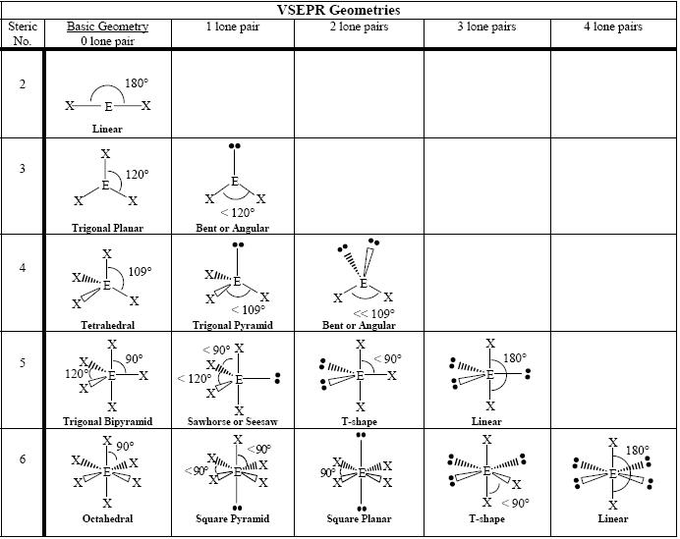
\includegraphics[width=\textwidth]{resources/vsepr-table.png}

\subsection{Polarity}
The "polarity" of a molecule refers to a vector of charge flowing throughout.
The polarity of a molecule depends on the polarity of the bonds in the molecular
geometry.

There is a distinction between the molecular diople and the individual component
bond dipoles that is illustrated below.

\begin{equation}
\vec{\mu}_{\text{mol.}} = \sum_{i=1}^{n} \vec{\mu}_{i}
\end{equation}

To determine the polarity of a molecule, implement the following processes:

\begin{enumerate}
  \item Draw a Lewis structure.
  \item Determine the molecular geometry.
  \item Determine the polarity of the individual bonds. (Positive points to
    negaitve).
  \item Draw bond dipoles as vectors.
  \item Sum the vectors and draw the molecular dipole.
\end{enumerate}

\subsection{Hybridization}
Orbitals on a single atom will hybridize to form new orbitals. These hybridized
orbitals will be combinations of valence level orbitals, which determines the
shape of a molecule.

Some hybridizations are listed below.

\begin{table}[]
\centering
\begin{tabular}{|l|l|l|}
\hline
\textbf{electron pair geometry} & \textbf{orbitals} & \textbf{hybridization} \\ \hline
linear                          & $s,p$             & $sp$                   \\ \hline
trigonal planar                 & $s,p,p$           & $sp^3$                 \\ \hline
tetrahedral                     & $s,p,p,p$         & $sp^3$                 \\ \hline
trigonal bipyramidal            & $s,p,p,p,d$       & $sp^3d$                \\ \hline
octahedral                      & $s,p,p,p,d,d$     & $sp^3d^2$              \\ \hline
\end{tabular}
\end{table}

\chapter{Unit 5}

\chapter{Unit 6}
\section{Integration by Parts}
To integrate using parts, pick a $u$ and a $dv$ from the origianl integral. The
$dv$ ideally should be something that is easy to integrate, while the $u$ should
be easy to differentiate.

Once selected, simply apply the formula to yield your answer. You may have to do
parts more than once, or have the recursive case where the original integral
comes up again, and you have to move it to one side.

\begin{equation}
  \int u dv = uv - \int v du
\end{equation}

\section{Powers of Trigonometric Expressions}
\subsection{$\int \cos^n\theta\sin^m\theta d\theta$}
\begin{description}
  \item[$n$ or $m$ odd] convert all but one of that function to the other using
    a trigonometric identity. The remaining power is the $d\theta$.
  \item[$n$, $m$ both even] use a power reducing formula.
\end{description}

\subsection{$\int \sec^n\theta\tan^m\theta d\theta$}
\begin{description}
  \item[$n$ is even] convert all but one $\sec^2\theta$ to $\tan$s using a
    trigonometric identity. The remaining $\sec^2\theta$ will be your $d\theta$.
  \item[$n$ is odd] convert all but one to $\sec\theta$, saving a
    $\sec\theta\tan\theta$.
  \item[$n=0$, $m$ is anything] convert one $\tan^2\theta$ to $\sec^2\theta-1$
\end{description}

\subsection{Base-case}
If the trigonometric power expression you have is none of the above, you have to
convert everything to $\sin$s and $\cos$s and simplify from there.

\section{Triginometric Substitution}
You can substitute three cases of integrals into a triangle and then simplify
in terms of $\theta$. Integrate with respect to $d\theta$ and then convert your
answer back in terms of $x$, $y$, or $z$ using the original triangle.

\begin{align}
  \sqrt{a^2-u^2} &\to \sin\theta = \frac{u}{a} \\
  \sqrt{a^2+u^2} &\to \tan\theta = \frac{u}{a} \\
  \sqrt{u^2-a^2} &\to \sec\theta = \frac{u}{a}
\end{align}

\section{Partial Fractions}
If you have a integral where the denominator is factorable (or can be split to
become factorable) then you can use partial fractions.

\begin{equation}
  \int \frac{p(x)}{q(x)} dx = \int {\frac{A}{x}+\frac{B}{(x+1)}+\ldots\; } dx
\end{equation}

There are a few rules when dealing with expanding the denominator to use partial
fractions.
\begin{itemize}
  \item If you have a factor in the form $(px^2+q)$, the numerator is in the
    form $(Ax+B)$.
  \item If you have a factor in the form $(px+q)$ then then numerator is in the
    form of $A$.
\end{itemize}

To solve...
\begin{enumerate}
  \item Make the denominator factor-able.
  \item Break apart the partial fraction.
  \item Create the basic equation.
  \item Isolate terms by power.
  \item Solve the system.
  \item Integrate each part.
\end{enumerate}


\end{document}
